\documentclass{article}
\usepackage{amsmath}
\usepackage{tikz}
\usetikzlibrary{fit,tikzmark}
\tikzset{submatrix/.style = {draw, rectangle, rounded corners,
  fill=yellow}, inner sep=2pt}
\pagestyle{empty}
\begin{document}
\begin{tikzpicture}[overlay, remember picture]
  \node (m) [submatrix, fit={([yshift={1.5ex}]pic cs:m1) (pic cs:m2)}] {};
  \node (n) [submatrix, fit={([yshift={1.5ex}]pic cs:n1) (pic cs:n2)}] {};
  \draw [->] (m.south east) to[bend right=20] (n.south west);
\end{tikzpicture}
\[
  \begin{pmatrix}
       1 & 2 & 3 \\
       4 & \tikzmark{m1}5 & 6 \\
       7 & 8 & 9\tikzmark{m2}
  \end{pmatrix}
  \xrightarrow{\text{Transpose}}
  \begin{pmatrix}
     1 & 4 & 7 \\
     2 & \tikzmark{n1}{5} & 8 \\
     3 & 6 & 9\tikzmark{n2} 
  \end{pmatrix}
\]
\end{document}
